\documentclass
%[handout]
{beamer}
\usepackage{folien}
\usepackage[utf8]{inputenc}
\usepackage{graphicx}
\usepackage{alltt}
\usepackage{myrules}

%\renewcommand\comment[1]{}

\author{Benus Becker}
\title{EasyOCaml}
\subtitle{}
\date{28. Januar 2009}
\institute{Universität Freiburg}% \\ Institut für Informatik \\ Abtg.\ für Programmiersprachen}
\keywords{ocaml, types}
\subject{Studienarbeit}

\begin{document}

\frame{\titlepage}

\begin{frame}{Motivation}
  \centerline{\tt let f b x = let y = if b then x in x + y ;;}
  \pause
  \begin{description}
    \item[Objective Caml]\ \\
      \texttt{\# let f b x = let y = if b then x in \underline x + y ;;\\
      Error: This expression has type unit but is here used with type int}
      \pause
    \item[EasyOCaml]\ \\
      \only<+>{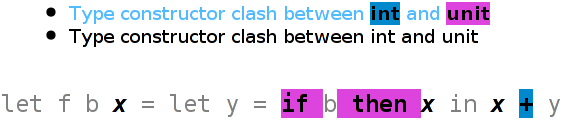
\includegraphics[rotate=90,width=0.75\textwidth]{mightadd}}
      \only<+>{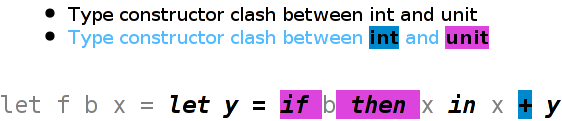
\includegraphics[rotate=90,width=0.75\textwidth]{mightadd1}}
  \end{description}
\end{frame}

\begin{frame}{Ziele}
  \begin{itemize}
    \item Fehlermeldungen verbessern
      \begin{itemize}
        \item Parser
        \item Typchecker
      \end{itemize}
    \item didaktische Hilfsmittel
      \begin{itemize}
        \item Einschränkungen der Syntax
        \item Bereitstellung von Code
      \end{itemize}
    \item Integration in das existierende OCaml System
      \begin{itemize}
        \item Nutzen der existierenden Codegenerierung
        \item Zugriff auf vorhandene Programmbibliotheken
      \end{itemize}
  \end{itemize}
\end{frame}

\begin{frame}{Verwandte Projekte}
  \begin{description}
    \item[Haack \& Wells (2004)]\ \\
      \begin{itemize}
        \item Constraint-basiertes Typchecken von MiniML
        \item minimale, ausreichende Begründung der Fehler
      \end{itemize}
    \item[Helium]\ \\
      \begin{itemize}
        \item Haskell Implementation ``für Anfänger''
        \item Hinweise zum Lösen der Typfehler
      \end{itemize}
    \item[DrScheme]\ \\
      \begin{itemize}
        \item Standard IDE für Programmierkurse in Scheme
        \item einfacher Debugger
        \item Language Levels und Teach Packs
      \end{itemize}
  \end{description}
\end{frame}

\begin{frame}{Unterstützte Sprache}
  Caml$_{-m}$: Caml ohne Moduldeklarationen
  \begin{description}
    \item[Werte]
      Primitive, Tupel, Listen, Arrays, Varianten, Records, Funktionen, Ausnahmen.
    \item[\emph{Structure items}]
      Typ-, Ausnahmen-, Wertdeklarationen und Expressions.
    \item[\emph{Pattern}]
      Geschachtelt auf alle möglichen Werte.
    \item[Ausdrücke]
      Konstruktoren, Ausnahmebehandlung, Konditionale, Abstraktionen, Typannotationen.
  \end{description}
  \comment{Einschränkbar durch Language Levels}
  \comment{Alle Teile der stdlib ohne format typbar}
\end{frame}

\begin{frame}{Einbettung in OCaml}
  Ablauf von EasyOCaml
  \begin{itemize}
    \item Kommandozeilenparameter: \texttt{-easy}, \texttt{-easyerrorprinter},
      \texttt{-easylevel}, \texttt{-easyteachpack}
    \item Modifikation des Parsers, Laden von Teach Packs
    \item Syntaxanalyse mit Camlp4
    \item Constraintbasierte Typrekonstruktion
    \item Zurückführung in den Compiler bzw.\ die REPL
      \comment{bisher typt Ocaml selbst erneut}
  \end{itemize}
\end{frame}

\begin{frame}{Typchecker}
  \framesubtitle{Haack \& Wells, 2004}
    \texttt{\# let f b x y = x + \underline{if b then y} ;;\\
   * Type error: Type constructor clash between int and unit.
   Slice: .. + if .. then .. else () ..}
   \comment{
     $\mathcal W$ erzeugt und löst Constraints gleichzeitig: Keine Nachprüfung möglich \\
     Trennung von Generierung und Lösung
   }
  \begin{itemize}
    \item Ziele
      \begin{itemize}
        \item mehrere Fehler auf einmal berichten
        \item Fehler sind minimal und vollständig\comment{definieren}
      \end{itemize}
      \pause
    \item Haack \& Wells' Typchecker für MiniML
      \begin{enumerate}
        \item Generierung von Constraints
        \item Lösen von Contraints
        \item Aufzählen der Fehler
        \item Minimierung der Fehler
      \end{enumerate}
      \pause
    \item Gleichzeitig mit Constraintgenerierung: Unbekannte Variablen erkennen
  \end{itemize}
\end{frame}

\begin{frame}{Typchecker}
  \framesubtitle{Erweiterungen für EasyOCaml}
  \begin{itemize}
    \item Syntaktische Kategorien
      \begin{description}
        \item[Deklarationen] $\Delta;\ strit \Downarrow_s \langle \Delta,\ C,\ u\rangle$
        \item[Ausdrücke] $\Delta;\ lexp \Downarrow_e \langle ty,\ C,\ u\rangle$
        \item[Pattern] $\Delta;\ pat \Downarrow_p \langle ty,\ C,\ b\rangle$ 
      \end{description}
    \item Typen: Varianten, Records \\ Beispiel
%\inferrule[Variant] {
%  \Delta\onvar(K) = \langle ty_r,\ [ty_{a,1},\ \dots,\ ty_{a,n}]\rangle \\
%  \etyjudge \Delta {lexp_i} {ty_i} {C_i} {u_i} \text{ for } i=1,\dots,n \\
%  C_0 = \{a \xlongequal l ty_r \} \cup \{ ty_i \xlongequal l ty_{a,i}\ |\ i=1,\dots,n \} \\
%  a \fresh
%} {
%  \etyjudge \Delta {(K\  lexp_1\ \dots\ lexp_n)^l} a {\bigcup_{i=0}^n C_i} {\bigcup_{i=1}^n u_i}
%}
      \[\inferrule[Record Access]
      {
       \etyjudge \Delta {lexp} {ty} C u \\
       \Delta\onrecord(f) = \langle ty_f,\ ty_,\ \cdot \rangle \\
       C_0 = \{a \xlongequal {l} ty_f,\ ty \xlongequal l ty_r\} \\
       a \text{ fresh}}
       {\etyjudge \Delta {(lexp\code{.}f)^l} a {C_0 \cup C} u}\]
  \end{itemize}
  \comment{mehr mögliche Fehler}
\end{frame}

\begin{frame}{Typannotationen}
  $(lexp : ct)$
  \begin{itemize}
    \item $lexp$ und Kontext werden unabhängig getypt
    \item Validität der Annotation wird nachträglich geprüft
  \end{itemize}
\[\inferrule[Type-Annot]{
\etyjudge \Delta {lexp} {ty} {C_0} u \\
C_1 = \{a \xlongequal l ty',\ ty \succcurlyeq^l ct\} \\
a \text{ fresh} \\
ty' \text{ is a fresh instance of } ct \\
}{
  \etyjudge{\Delta}{(lexp : ct)^l}{a} {C_0 \cup C_1} {u}
}\]
      \comment{Annotation wird als korrekt angenommen}
\end{frame}

\begin{frame}{Beispiel: Generierung von Typconstraint}
  \texttt{x + if b then y}
\end{frame}

\begin{frame}{Fehlerbehandlung}
  Drei Klassen von Fehlern
  \begin{itemize}
    \item Einfach: Meldung nach Typrekonstruktion
    \item Schwer: Meldung nach Constraintgenerierung
      \comment{Analyse der Validität von Varianten, Records, Typkonstruktionen}
    \item Fatal: Sofortige Meldung
  \end{itemize}
  Anpassung der Fehlermeldungen
  \begin{itemize}
    \item Internationalisierung der Fehlerbeschreibung
      \comment{Gesteuert durch Umgebungsvariable}
    \item Formatierung für unterschiedliche Ausgaben (Plugin)
      \comment{Funktionen werden registriert in dynamisch geladenem Code}
  \end{itemize}
\end{frame}

\begin{frame}{Language Levels und Teach Packs}
  \begin{itemize}
    \item Definition und einfache Auslieferung verfügbarer Sprachkonstrukte und
      vordefiniertem Codes
      \comment{um die Sprache an Übungen und Inhalt von Kursen anzupassen}
    \item Interface
      \begin{description}
        \item[Sprachspezifikation]\ \\
          \begin{itemize}
            \item Deaktivierung von Optionen für die nicht-terminale Deklaration,
              Ausdruck, Pattern im Parser
            \item[$\Rightarrow$]direkte Manipulation des Parsers
              \comment{keine Meldungen bzgl.\ unbekannter Kategorien}
            \item für jede Benutzung unabhängig
          \end{itemize}
          \comment{
            Patterns können anders in try-with und match-with sein \\
            Parser wird auf den ggT eingeschränkt, anderes wird danach getestet
          }
        \item[Vordefinierter Code] 
          Liste von (zu öffnenden) Modulen
          \comment{
            Language Levels definieren Sprache und vorgegebenen Code \\
            Teach Packs enthalten nur Code und können Ll.s erweitern
          }
      \end{description}
  \end{itemize}
\end{frame}

\begin{frame}{Änderungen am Parser}
  EasyOCaml parst mit Camlp4 Parser
  \begin{itemize}
    \item hart kodierte Beschreibung
    \item Streamparser erlauben nur Zeichenketten als Information
      \singleitem[$\Rightarrow$]{\tt exception Stream.Error of string}
  \end{itemize}
  Lösung (?)
  \begin{itemize}
    \item interne Struktur der Zeichenkette: \texttt{"<msg>\textbackslash 000<mshl>"}
    \item Wiederherstellung des ``gemarshalten'' Fehlers in der Interfacefunktion 
  \end{itemize}
\end{frame}

\begin{frame}{Bisherige und weitere Entwicklung}
  \begin{itemize}
    \item[\checkmark] Typchecker für Teilsprache von OCaml
    \item[\checkmark] Internationalisierte und anpassbare Fehlermeldungen
    \item[\checkmark] Hilfsmittel für die Lehre mit OCaml
    \item[\checkmark] Integration in original Compiler und REPL
    \item[\checkmark] Anpassbare Fehlermeldungen für den Parser
    \item[\checkmark] HTML Fehlerausgaben
    \item[\checkmark] Portierung auf OCaml 3.11
    \pause
    \item Integration in DrOCaml oder Camelia
    \item Heuristiken/Tips zum Lösen von Fehlern
    \item Fehlermeldungen mit mehr Informationen versehen
    \item selbstdokumentierende Language Levels und Teach Packs
    \item dynamisch getypter Interpreter
  \end{itemize}
\end{frame}

\begin{frame}{Fazit}
%  \begin{itemize}
%  \end{itemize}
  \begin{itemize}
    \item Zweigeteilt: Arbeit am Typchecker -- Integration in OCaml
    \item moderne Forschungsergebnisse (Haack \& Wells) anwenden
    \item OCaml verbessern und open source zu arbeiten
  \end{itemize}
\end{frame}

\begin{frame}{Quellenangaben}
  \nocite{leroy2008}
  \nocite{haackwells04}
  \nocite{helium-hw03}
  \nocite{Felleisen98thedrscheme}
  \bibliographystyle{chicago}
  \clearpage\bibliography{easyocaml}
\end{frame}

\end{document}
